% Introduction. Source: HTML §1 (refs/internal/html-report/amphionasr-report-en.html);
% 1.0 facts: AmphionASR 1.0 PDF §5.4 (amphion2026amphionasr).
% Structure modelled on the 1.0 report's introduction (problem scenario ->
% shortfall -> contributions), per AGENTS.md rule 6.

\section{Introduction}
\label{sec:intro}

\begin{figure}[t]
  \centering
  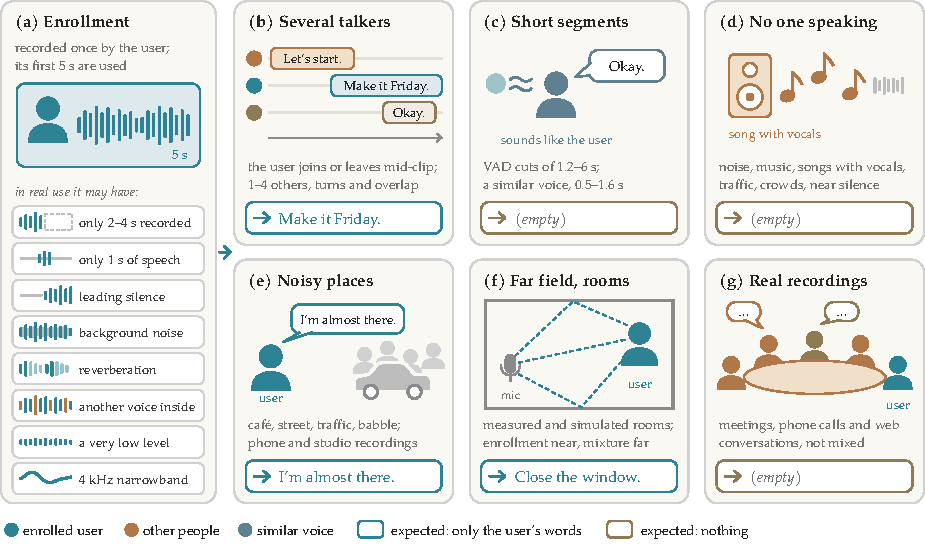
\includegraphics[width=\linewidth]{figures/scenarios.pdf}
  \caption{Situations from real use that \tsbench covers, one panel per section of the benchmark. (a)~The enrollment, recorded once by the user, of which the first 5\,s are used, and the degradations it may have in real use. (b)--(g)~Situations in the recording, each with the output expected from a TS-ASR model: only the enrolled user's words, or nothing when the user does not speak. VAD: voice activity detection. Utterances are illustrative; the benchmark is in Mandarin.}
  \label{fig:scenarios}
\end{figure}

\begin{figure}[t]
  \centering
  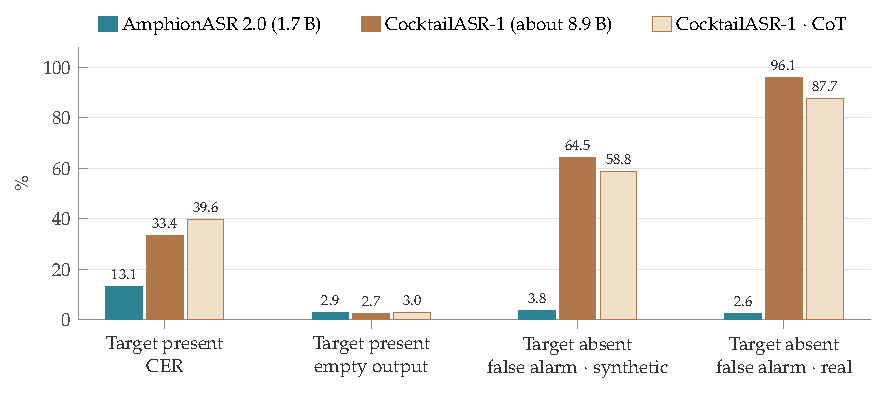
\includegraphics[width=\linewidth]{figures/main-results.pdf}
  \caption{Main results on \tsbench (\%, lower is better). The first two metric groups are computed on target-present samples only; the two false-alarm groups are computed on target-absent samples only, from synthetic scenes and from real meetings, calls and web conversations. All systems use the same audio, the first 5\,s of each enrollment and the same scoring.}
  \label{fig:teaser}
\end{figure}

SpeechLLMs connect an audio encoder to an autoregressive language model and are now used as general-purpose speech recognizers~\cite{shi2026qwen3asr}.
In meetings, at reception desks, in cars and on the street, however, a recording often contains several people speaking at once or in turn, and the user usually cares about only one of them.
Target-speaker automatic speech recognition (TS-ASR) addresses this case: the model receives an enrollment utterance of one person together with the recording, called the mixture, and transcribes only what that person says.
The task has two kinds of error that pull in opposite directions.
A \emph{miss} occurs when the enrolled speaker spoke but the model wrote nothing or only part of it; a \emph{false alarm} occurs when the enrolled speaker did not speak but the model transcribed someone else.
\Cref{fig:scenarios} shows the situations from real use covered by our benchmark, \tsbench; the correct output is either the enrolled user's words or nothing at all.

Our earlier AmphionASR~1.0~\cite{amphion2026amphionasr} combined retrieval-augmented hotwords, target-speaker selection, degradation robustness and whispered speech in one 1.7\,B model, and of these capabilities TS-ASR most needed work.
Its in-house test set was synthesized in the same way as its target-speaker training data.
That report gives a target-present WER of 13.02\%, measures the target-absent case only on 164 samples in which nobody speaks, and does not test what the model does when others speak while the enrolled speaker is silent.
The 1.0 report itself notes that these results do not establish competitiveness with dedicated TS-ASR systems under a matched protocol~\cite{amphion2026amphionasr}.
AmphionASR~2.0 therefore takes TS-ASR as its main target.

Improving TS-ASR first requires an evaluation that reflects real use.
Common evaluations of target speech extraction (TSE) and TS-ASR, such as WSJ0-2mix~\cite{hershey2016deep}, Libri2Mix~\cite{cosentino2020librimix} and LibriSpeechMix~\cite{kanda2020serialized}, overlay two or three read utterances.
The target is always present, the enrollment is another clean utterance of the same person, and metrics are computed only on target-present samples~\cite{zmolikova2019speakerbeam, zmolikova2023neural}.
WHAM!~\cite{wichern2019wham} and WHAMR!~\cite{maciejewski2020whamr} add noise and reverberation but keep the same mixing, and SpeechLLM work on TS-ASR mostly reports error rates on synthetic two-talker mixtures~\cite{zhang2025thinking, guo2024sqwhisper}.
These evaluations differ from real use in three ways:
\begin{itemize}[leftmargin=*, itemsep=2pt]
  \item \textbf{False alarms go unmeasured.} Without target-absent samples, a model that transcribes everyone can still score well; TSE research has also shown that evaluations assuming an always-active target hide false extractions~\cite{delcroix2022listen}.
  \item \textbf{No conversational structure.} Randomly overlaid read sentences lack the turn-taking, interjections, hand-overs, simultaneous starts and one- or two-word replies of meetings and conversations.
  \item \textbf{No real enrollment or recording conditions.} A user's enrollment may be short, noisy or contain another voice, and the recording may come from a far-field microphone or a phone call.
\end{itemize}

This report makes two contributions:
\begin{itemize}[leftmargin=*, itemsep=2pt]
  \item \textbf{\tsbench, a TS-ASR benchmark for real-world conditions} (\Cref{sec:benchmark}). It pairs every condition with target-present and target-absent samples and reports three metrics together. Its synthetic scenes are designed from errors observed in real use and change one factor at a time. Its real part comes from the test sets of public meeting and call corpora and from web conversations, without mixing. With 24{,}101 samples in 248 subsets, it shows that evaluations limited to a single talker, to samples with the target present or to silence lead to conclusions that do not hold in real conditions (\Cref{subsec:exp_conditions}). The benchmark will be released publicly.
  \item \textbf{AmphionASR~2.0, a TS-ASR model that also keeps plain and hotword recognition} (\Cref{sec:model,sec:data,sec:training}). The enrollment and the mixture pass separately through the convolutional downsampling of the audio encoder and are joined by a learnable separator before its Transformer layers, which attend globally. The training data are organized by scene type, each with target-absent counterparts that enroll another person, and include real meeting windows. Compared with Xiaomi-CocktailASR-1~\cite{zhang2026xiaomi} on \tsbench under the same protocol, AmphionASR~2.0 has about two fifths of its target-present CER and a false-alarm rate more than an order of magnitude lower when others talk and the enrolled speaker is silent (\Cref{fig:teaser}).
\end{itemize}

AmphionASR~2.0 is also initialized from Qwen3-ASR-1.7B~\cite{shi2026qwen3asr} but differs from 1.0 in two ways: all of its parameters are fine-tuned, and the enrollment is placed inside the audio encoder.
In 1.0, the enrollment is encoded separately and enters the language model as its own span of audio embeddings.
Version~2.0 does not include the hotword-retrieval module or the whispered-speech training of 1.0, and this report does not evaluate those two capabilities.
